% A section containing the results. In case the project is a control-oriented project this should include plots of measurement signals, reference signal, and control signal. If the project is more of a real-time nature then this section could contain measurement results of different type.

%PLOTTAR FÖR SEQUENCE, FÖRKLARA NÄR VAD HÄNDER \\
%klart, eller?
FÅ PLOTTAR ATT LIGGA RÄTT I DOKUMENTET

In the figures, the top graph shows the reference values and measured values for the angle of the beam. 
The middle graph shows the same values for the position of the ball. 
Reference values are shown in black, while measured values are red. 
The bottom plot shows the control signal.

Figures \ref{fig:stepresponsebeam} and \ref{fig:stepresponseball} show the step responses for the beam angle and the ball position, respectively. 
The beam step response shows a large overshoot but a quick settling.
The ball step response also shows a quite large overshoot, while also being quite slow.
As the plots show, the control signal has a tendency to be noisy.

Figures \ref{fig:topickupposition}-\ref{fig:weighbandthrowlargeball} show plots for different parts of the sequence described in section \ref{sec:controller_structure}.
As can be seen in for example figure \ref{fig:weighmediumball}, no great precision is needed when weighing the ball. See section \ref{sec:ball_weighing}.

\begin{figure}[h]
\centering
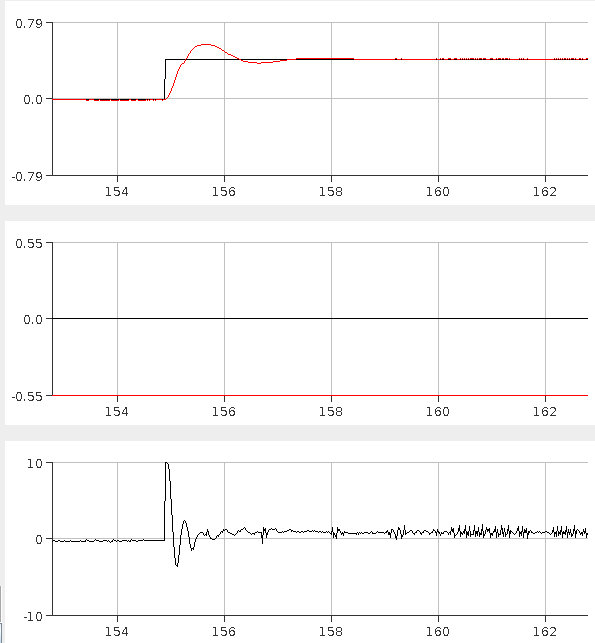
\includegraphics[width=0.7\textwidth]{figures/stepresponsebeam-crop.png}
\caption{Step response for the beam angle.}
\label{fig:stepresponsebeam}
\end{figure}

\begin{figure}[h]
\centering
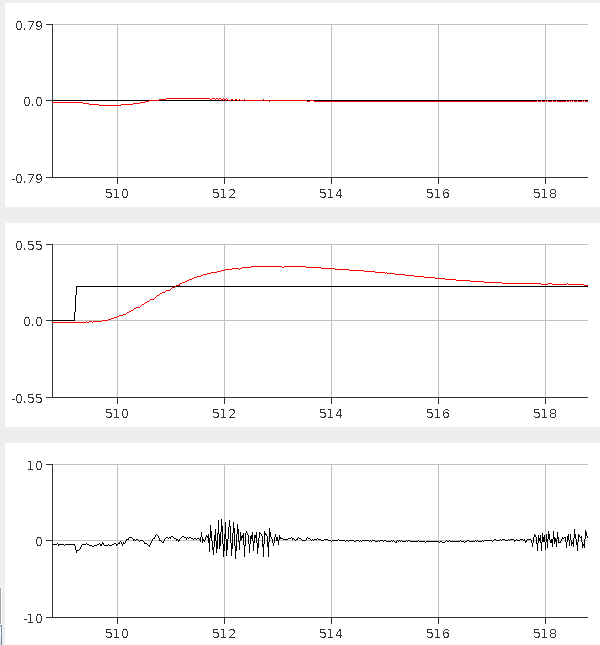
\includegraphics[width=0.7\textwidth]{figures/stepresponseball1-crop.png}
\caption{Step response for the ball position. Notice the noisy control signal.}
\label{fig:stepresponseball}
\end{figure}

\begin{figure}[h]
\centering
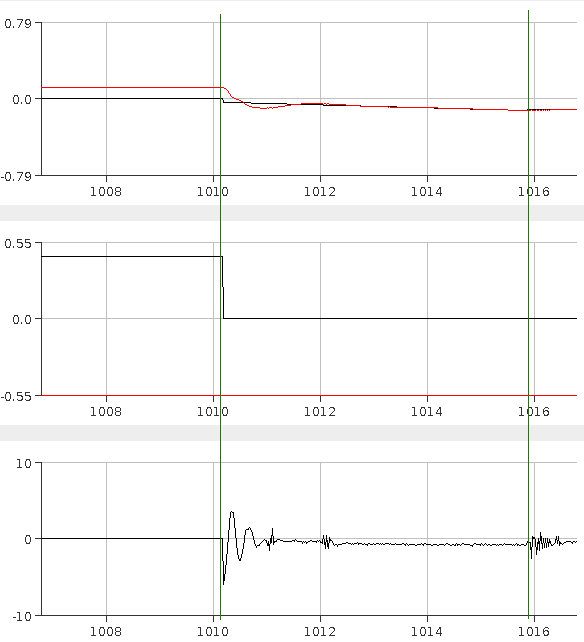
\includegraphics[width=0.7\textwidth]{figures/topickupposition-crop.png}
\caption{Controlling the beam angle to search for the appropriate pickup position, as described in section \ref{sec:ball_catching}. The process is started at the first line in the graph, and the LED is detected around the second.}
\label{fig:topickupposition}
\end{figure}

\begin{figure}[h]
\centering
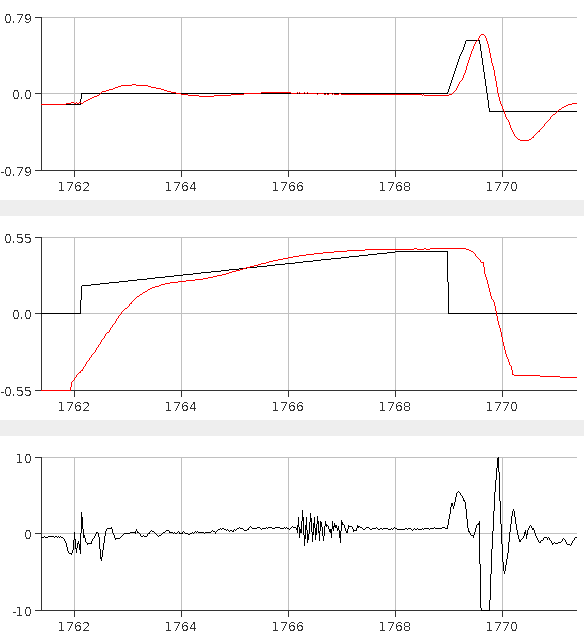
\includegraphics[width=0.7\textwidth]{figures/weighandthrowsmallball-crop.png}
\caption{Weighing and throwing the small ball. The ball enters the beam at the first line, and is finished being weighed around the second one. After being stabilized (See section \ref{sec:small_ball_delivery}), it is thrown at the third line.}
\label{fig:weighandthrowsmallball}
\end{figure}

\begin{figure}[h]
\centering
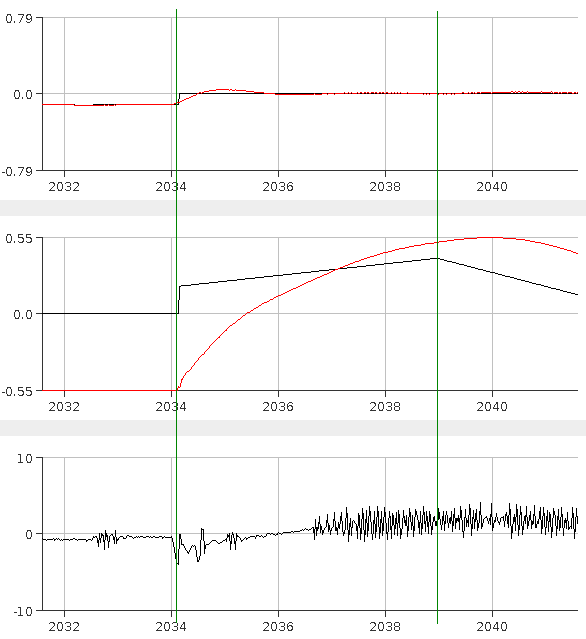
\includegraphics[width=0.7\textwidth]{figures/weighmediumball-crop.png}
\caption{Weighing the medium ball, and the beginning of moving it to prepare for a throw. The ball is detected at the first line, and is finished being weighed at the second.}
\label{fig:weighmediumball}
\end{figure}

%kanske inte jätteintressant?
\begin{figure}[h]
\centering
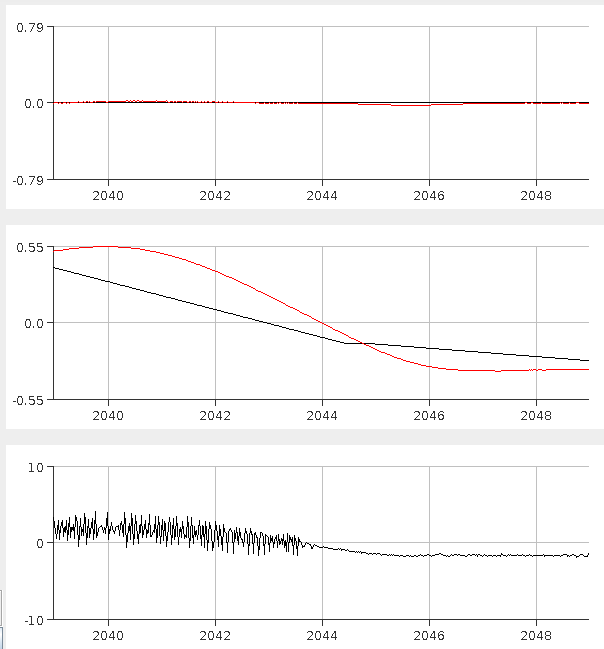
\includegraphics[width=0.7\textwidth]{figures/movemediumball-crop.png}
\caption{Moving the medium ball to throwing position.}
\label{fig:movemediumball}
\end{figure}

\begin{figure}[h]
\centering
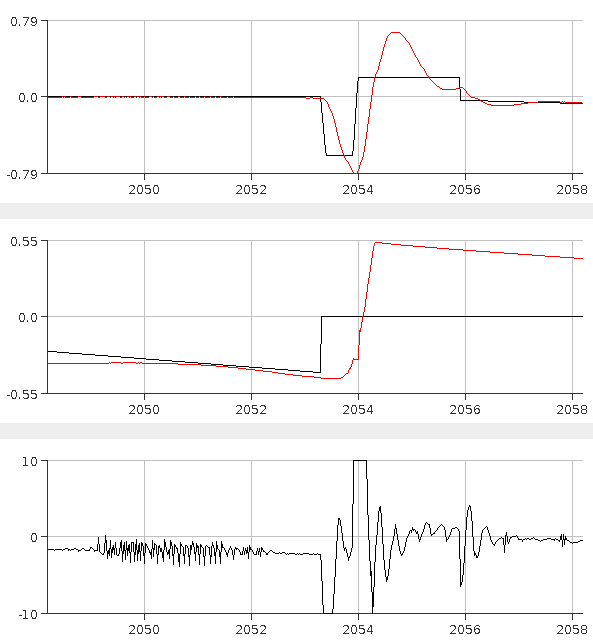
\includegraphics[width=0.7\textwidth]{figures/throwmediumball-crop.png}
\caption{The medium ball arriving at the throwing position, and then getting thrown, at the time point specified by the line.}
\label{fig:throwmediumball}
\end{figure}

\begin{figure}[h]
\centering
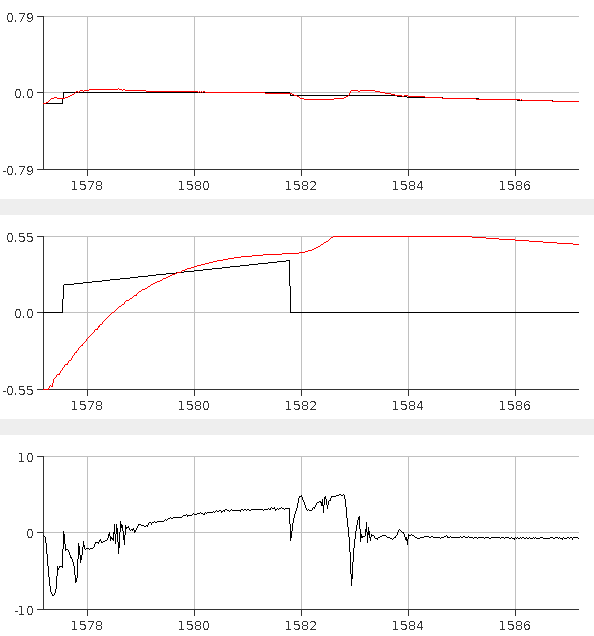
\includegraphics[width=0.7\textwidth]{figures/weighanddroplargeball-crop.png}
\caption{Weighing and dropping the large ball. The ball enters the beam at the first line, and is finished being weighed at the second, after which it is dropped.}
\label{fig:weighbandthrowlargeball}
\end{figure}



